% Copyright 2026 Sreeram Anil
% SPDX-License-Identifier: CC-BY-4.0
% =============================================================================
%  Coulomb counting (ampere-hour integration) — baseline family
% =============================================================================
\chapter{Coulomb Counting (ampere-hour integration)}
\label{ch:coulombcounting}

\section*{At a glance}
\begin{tabular}{@{}l>{\raggedright\arraybackslash}p{0.76\textwidth}@{}}
Family & baselines \\
Header & \texttt{include/estkit/battery/baselines.hpp} \\
Registered name & \texttt{CoulombCounting} \\
State dimension & $n_x = 4$ propagated open-loop; only $\soc$ is reported \\
Cost per step & $\mathcal{O}(n_x)$, $\approx 79$\,ns/step measured, no heap, no feedback \\
Primary references & \cite{ng2009coulomb,plett2015bms1,lin2018sensorbias} \\
\end{tabular}

\section{Motivation and relevance}
Coulomb counting is the open-loop integration of the measured current, and it is worth studying in
its pure form for three reasons. It is the \emph{time update} of every Kalman filter in
Parts~III--VI --- the $\soc$ row of the ECM model (Chapter~\ref{ch:ecm}) is exactly
\eqref{eq:cc-recursion}, so whatever afflicts it also afflicts the EKF's prediction step; the
difference is only that a filter gets to correct it. Its error is \emph{analytic}: alone among the
methods in this report, its end-of-mission error is a closed-form function of the current-sensor
gain and offset, the elapsed time, the throughput and the capacity error, and \eqref{eq:cc-drift}
is the quantitative baseline for the \code{current\_bias} and \code{aged\_cell} columns of every
results table. And it is the fallback when a voltage channel fails or the cell sits on an OCV
plateau, so a certification argument needs a defensible statement about it. Ng
et~al.~\cite{ng2009coulomb} made the essential point --- the practical limit is sensor calibration
and capacity knowledge, not the integration --- and it is why no production BMS ships it alone.

\section{Problem statement and assumptions}
The method estimates only $\soc$, from the current channel; the voltage is accepted and ignored, and
a predicted voltage is reported so that the residual diagnostic of \S\ref{sec:me-residual} is
available.
\begin{assumption}\label{as:cc-all}
(i) the capacity $Q$ is known and constant; (ii) the current sensor is calibrated,
$i^{\text{m}} = i$ up to zero-mean noise; (iii) $\hat\soc_0 = \soc_0$.
\end{assumption}
All three are violated by the benchmark on purpose. Item~(iii) is the sharpest: there is no
feedback, so an initial error is never removed.

\section{Derivation}
With the discharge-positive convention, coulombic efficiency $\eta(i)=1$ on discharge and $\eta_c$
on charge, and a zero-order hold on the current over $[t_{k-1},t_k)$,
\begin{equation}
\hat\soc_{k} \;=\; \hat\soc_{k-1} \;-\; \frac{\eta(i^{\text{m}}_{k-1})\,\dt}{3600\,\hat Q}\; i^{\text{m}}_{k-1},
\label{eq:cc-recursion}
\end{equation}
$\hat Q$ being the capacity in \si{\ampere\hour} the estimator was told. The implementation obtains
this by calling the model's $f$, so $v_1,v_2,h$ propagate open-loop alongside $\soc$ and make the
diagnostic voltage $\hat v_k = h(\xminus_k,\vu_k)$ meaningful.

Let $e_k = \hat\soc_k - \soc_k$, let the true capacity be $Q = \hat Q(1-\delta)$ with $\delta$ the
fractional capacity loss, and let the current channel be $i^{\text{m}} = \kappa i + b_i + n_k + q_k$
(gain, offset, noise, quantisation residual; Chapter~\ref{ch:datasets}). Integrating
\eqref{eq:cc-recursion} over a mission of duration $T$ with throughput
$A_h = \frac{1}{3600}\int_0^T i\,\mathrm{d}t$ in \si{\ampere\hour}, and subtracting the true
evolution $\soc(T)-\soc(0) = -A_h/Q$, gives
\begin{equation}
\boxed{\;
e(T) \;=\; \underbrace{e(0)}_{\text{initial}}
\;-\;\underbrace{\frac{(\kappa-1)\,A_h}{\hat Q}}_{\text{gain}}
\;-\;\underbrace{\frac{b_i\,T/3600}{\hat Q}}_{\text{offset}}
\;-\;\underbrace{\frac{\mathcal{N}}{\hat Q}}_{\text{noise}}
\;+\;\underbrace{\frac{A_h\,\delta}{\hat Q(1-\delta)}}_{\text{capacity}} \; }
\label{eq:cc-drift}
\end{equation}
with $\mathcal{N} = \frac{1}{3600}\int_0^T(n+q)\,\mathrm{d}t$. Four consequences follow.

\emph{Gain scales with throughput, offset with time.} A \SI{19}{\minute} hover-hold and a
\SI{48}{\minute} fixed-wing mission remove almost the same charge, so their gain-induced errors are
equal, but the offset term is $2.5\times$ larger on the longer one. A sensor specified only by its
full-scale accuracy cannot be assessed without the duty cycle.

\emph{The random part is negligible.} $\mathcal{N}$ is a random walk of standard deviation
$\sigma_i\sqrt{\dt\,T}/3600 = \SI{1.97e-4}{\ampere\hour}$ over the eVTOL mission --- \SI{0.004}{\percent}
of SOC, two orders below the deterministic terms --- and quantisation adds
$q_i/\sqrt{12} = \SI{2.9}{\milli\ampere}$~\cite{widrow2008quantization} and a further
\SI{0.0002}{\percent}. Ampere-hour integration does not accumulate sensor noise; it accumulates
sensor \emph{bias}. The only quantisation mechanism that matters is the degenerate one, where a
constant current sits at a fixed distance from a code boundary and the rounding residual becomes a
DC offset of up to $q_i/2 = \SI{5}{\milli\ampere}$, worth \SI{0.056}{\percent} of SOC per mission.

\emph{The capacity term has the dangerous sign.} It is positive for $\delta>0$: an aged cell, whose
true capacity is smaller than the estimator believes, yields an estimate that is too \emph{high}.
Coulomb counting on an aged cell is systematically optimistic --- the failure direction that matters
on final approach. When $\delta$ accumulates during the mission as $\delta\propto A_h^{z}$ with
$z=0.55$, the integral replaces the product and the term becomes $\delta A_h/\bigl((1+z)\hat Q\bigr)$.

\emph{There is no forgetting.} $e(0)$ appears with coefficient one for all $T$, so
\code{init\_error} is not a convergence test for this method but a demonstration that it has no
convergence.

\paragraph{Quantitative check.} Substituting the nominal eVTOL numbers
($A_h = \SI{3.763}{\ampere\hour}$, $T=\SI{2010}{\second}$, $\hat Q = \SI{5}{\ampere\hour}$,
$\kappa = 1.005$, $b_i = \SI{20}{\milli\ampere}$, in-flight fade $\delta = \SI{0.327}{\percent}$)
into \eqref{eq:cc-drift} gives $-0.376-0.223+0.159 = -\SI{0.44}{\percent}$, against a measured final
error of $-\SI{0.443}{\percent}$. For \code{current\_bias} it predicts
$-1.505-2.792+0.159 = -\SI{4.14}{\percent}$ against a measured $e_{\max}$ of \SI{4.14}{\percent};
for \code{aged\_cell}, $-0.60+13.28 = +\SI{12.7}{\percent}$ against \SI{12.90}{\percent}. The formula
is not an approximation of the benchmark --- it \emph{is} the benchmark.

\section{Algorithm, application and implementation}
\begin{algorithm}[H]
\caption{Coulomb counting --- one sampling period}
\begin{algorithmic}[1]
\Require $\xhat_{k-1}$, stored $\vu_{k-1}$, new $i^{\text{m}}_k, T^{\text{m}}_k$ ($v^{\text{m}}_k$ unused)
\State $\vu_k \gets [\,i^{\text{m}}_k,\ T^{\text{m}}_k\,]^\T$
\If{$k>0$} \State $\xhat_k \gets f(\xhat_{k-1},\vu_{k-1})$ \Comment{open-loop; the $\soc$ row is \eqref{eq:cc-recursion}}
\EndIf
\State $\hat v_k \gets h(\xhat_k,\vu_k)$ \Comment{diagnostic only; never fed back}
\State $\vu_{k-1}\gets\vu_k$
\Ensure $\hat\soc_k = \xhat_k[\soc]$
\end{algorithmic}
\end{algorithm}

There is no tuning: the estimator uses \code{params} and \code{z0} from \code{EstimatorConfig} and
ignores $\mQ$, $\mR$ and $\sigma_{\soc_0}$ because it has no covariance; $\eta_c = 0.995$ acts only
on charge. The step is four multiply--accumulates, three exponentials (inherited from the shared
$f$) and one OCV lookup for the diagnostic voltage: \SI{79}{\nano\second}, the cheapest estimator in
the library. \code{sizeof} is \SI{4184}{\byte}, of which \SI{3872}{\byte} is the OCV
table used only for the diagnostic --- drop it and the method reduces to four scalars. The float32
build reproduces the double build to five digits; the one numerical caveat is long-horizon
accumulation, since over the 120-flight protocol the estimator performs $6\times10^{7}$ additions
and in binary32 a running sum near \num{0.5} absorbing increments of $10^{-5}$ is at the edge of
resolution. Compensated (Kahan) summation is the standard remedy and is not implemented because the
double build does not need it.

\section{Benchmark results}
% Copyright 2026 Sreeram Anil
% SPDX-License-Identifier: CC-BY-4.0
\begin{table}[H]\centering\footnotesize\setlength{\tabcolsep}{4pt}
\caption{CoulombCounting: cell-level benchmark on the eVTOL mission (mean over seeds; RMSE and max error in \% SOC; $t_\mathrm{conv}$: first time the error stays below 2\,\% for 60\,s, -- = never; EKF reference: steady-state RMSE of the plain EKF on the same data).}\label{tab:cell_CoulombCounting}
\begin{tabular}{llrrrrrcrr}\toprule
plant & scenario & RMSE & RMSE$_\mathrm{ss}$ & max & $t_\mathrm{conv}$ [s] & RMSE$_v$ [mV] & div. & EKF ref. & ns/step \\ \midrule
ECM & nominal & 0.28 & 0.36 & 0.44 & 0 & 3.41 & no & 0.05 & 79 \\
ECM & init\_error & 35.25 & 35.35 & 35.44 & -- & 8153.93 & yes & 0.05 & 79 \\
ECM & current\_bias & 2.44 & 3.20 & 4.14 & 0 & 28.12 & no & 0.61 & 81 \\
ECM & noise\_step & 0.28 & 0.36 & 0.44 & 0 & 3.41 & no & 0.12 & 80 \\
ECM & outliers & 0.28 & 0.35 & 0.44 & 0 & 3.39 & no & 0.21 & 80 \\
ECM & cold & 0.34 & 0.44 & 0.56 & 0 & 6.18 & no & 0.16 & 79 \\
ECM & hot & 0.20 & 0.24 & 0.28 & 0 & 2.25 & no & 0.03 & 80 \\
ECM & aged\_cell & 7.80 & 10.05 & 12.90 & 0 & 112.49 & no & 1.52 & 79 \\
ECM & param\_mismatch & 0.28 & 0.36 & 0.44 & 0 & 16.24 & no & 1.36 & 80 \\
ECM & sensor\_dropout & 0.28 & 0.36 & 0.44 & 0 & 3.41 & no & 0.46 & 79 \\
ECM & preisach & 0.28 & 0.36 & 0.44 & 0 & 9.24 & no & 0.20 & 80 \\
ECM & combined & 22.19 & 20.94 & 25.04 & -- & 1543.50 & no & 12.44 & 79 \\
\midrule
SPM & nominal & 0.36 & 0.47 & 0.60 & 0 & 10.26 & no & 3.73 & 75 \\
SPM & init\_error & 35.32 & 35.46 & 35.60 & -- & 8157.11 & yes & 3.81 & 75 \\
SPM & current\_bias & 2.52 & 3.31 & 4.30 & 0 & 29.47 & no & 5.69 & 75 \\
SPM & noise\_step & 0.36 & 0.47 & 0.60 & 0 & 10.26 & no & 3.30 & 74 \\
SPM & outliers & 0.36 & 0.46 & 0.60 & 0 & 10.24 & no & 1.99 & 74 \\
SPM & cold & 0.36 & 0.47 & 0.60 & 0 & 37.77 & no & 7.35 & 75 \\
SPM & hot & 0.36 & 0.47 & 0.60 & 0 & 8.84 & no & 2.16 & 73 \\
SPM & param\_mismatch & 0.36 & 0.47 & 0.60 & 0 & 18.69 & no & 3.13 & 75 \\
SPM & sensor\_dropout & 0.36 & 0.47 & 0.60 & 0 & 10.26 & no & 5.31 & 75 \\
\bottomrule\end{tabular}\end{table}

\begin{figure}[H]\centering
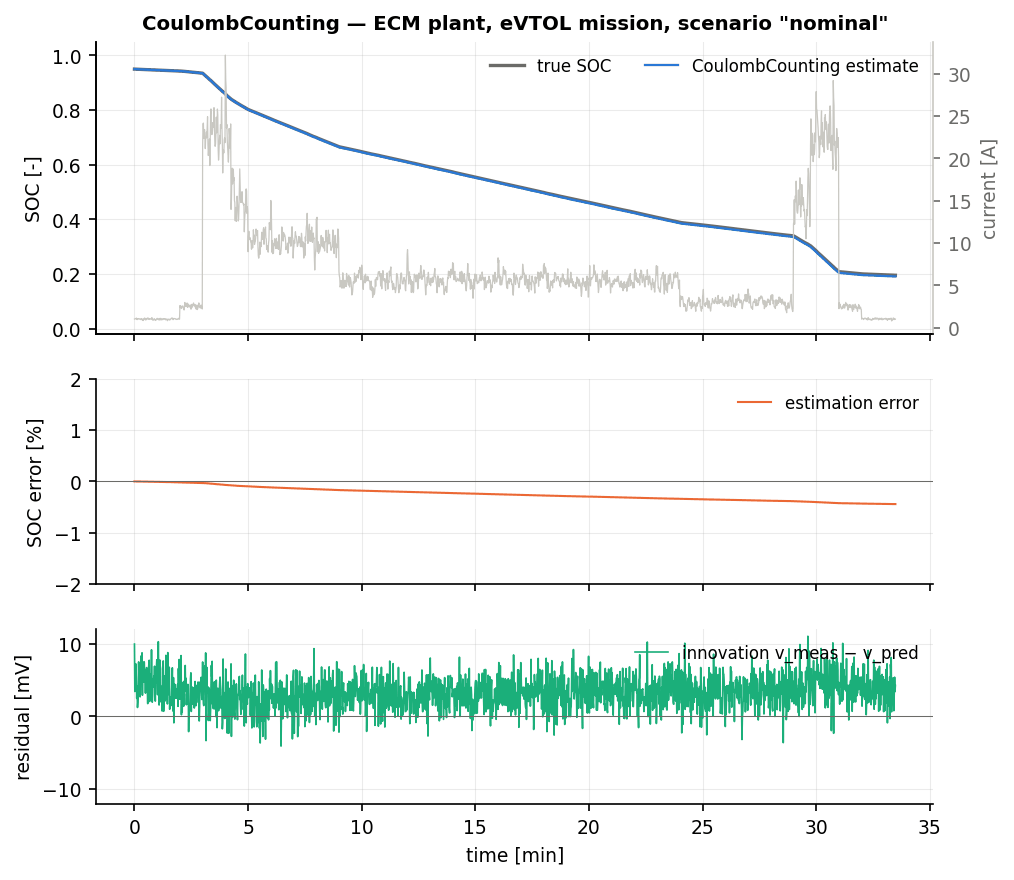
\includegraphics[width=0.78\textwidth]{figures/cell_CoulombCounting_nominal.png}
\caption{Coulomb counting on the nominal eVTOL mission: true and estimated SOC (top), estimation
error (middle), voltage residual (bottom). The error is a smooth monotone ramp --- the integral of a
constant bias --- with no visible noise-driven component, as \eqref{eq:cc-drift} predicts.}
\end{figure}
\begin{figure}[H]\centering
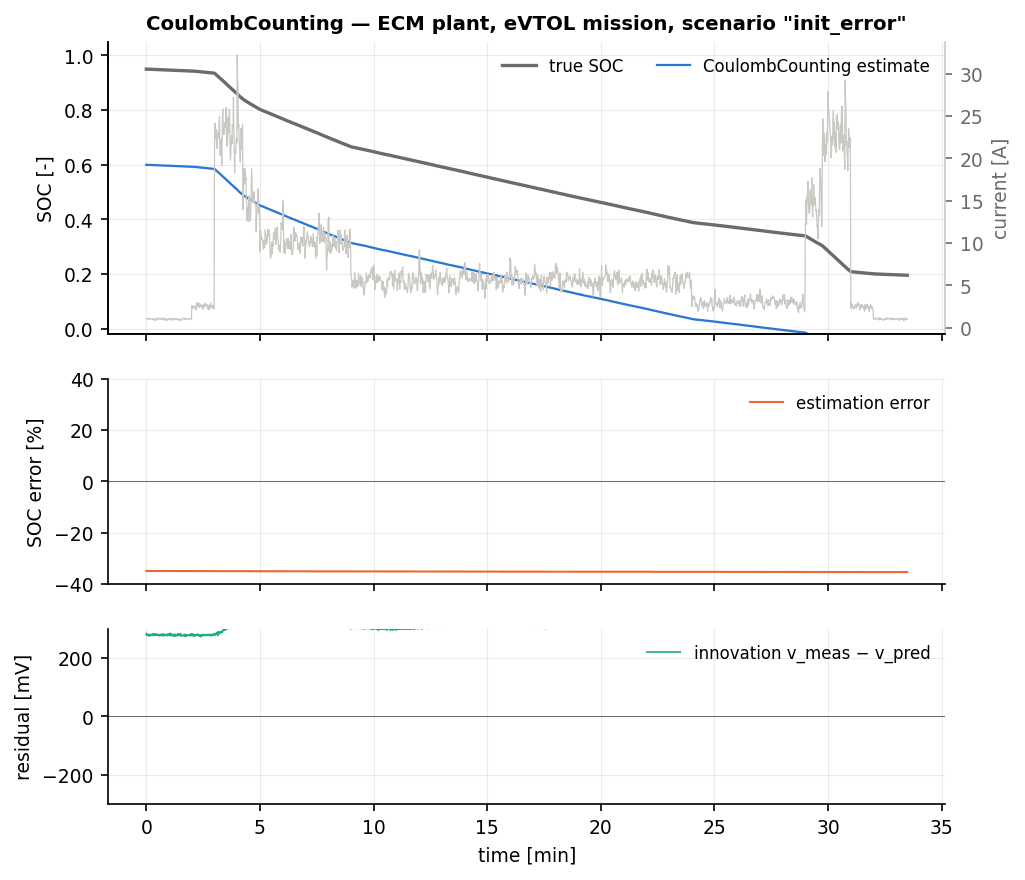
\includegraphics[width=0.78\textwidth]{figures/cell_CoulombCounting_init_error.png}
\caption{Coulomb counting with a $-35\,\%$ initial SOC error: the error is carried, unchanged, to
the end of the mission.}
\end{figure}

On the nominal eVTOL mission the method achieves $\text{RMSE}=0.28\,\%$ and
$\text{RMSE}_{\text{ss}}=0.36\,\%$ --- seven times the EKF's $0.05\,\%$, but in absolute terms
\SI{18}{\milli\ampere\hour} on a \SI{5}{\ampere\hour} cell. The steady-state figure \emph{exceeds}
the whole-run figure because the error grows monotonically; this inversion of the usual ordering is
the fingerprint of an uncorrected integrator, and it is the single clearest discriminator in the
whole results set --- every estimator with a working measurement update shows
$\text{RMSE}_{\text{ss}} \le \text{RMSE}$ on this scenario.

The scenarios split into three groups. Those that leave the current and the capacity alone ---
\code{noise\_step}, \code{outliers}, \code{sensor\_dropout}, \code{param\_mismatch} and
\code{preisach} --- give an estimate bit-identical to nominal ($0.36\,\%$ in every case, $0.35\,\%$
for \code{outliers}), because the voltage is not used. This is the one context in which the method
wins outright: $0.36\,\%$ against the EKF's $0.46\,\%$ on \code{sensor\_dropout}, against
$1.36\,\%$ on \code{param\_mismatch} and against the hybrid's $2.28\,\%$ on \code{preisach}
(Chapter~\ref{ch:coulombocvhybrid}). An estimator that does not look cannot be deceived. The
voltage-residual column still moves ($3.41\to\SI{16.24}{\milli\volt}$ under \code{param\_mismatch},
\SI{9.24}{\milli\volt} under \code{preisach}) --- a useful demonstration that $\text{RMSE}_v$
diagnoses the \emph{model} independently of the state.

Those touching the current channel or the capacity fail exactly as \eqref{eq:cc-drift} says:
\code{current\_bias} $3.20\,\%$ ($5.2\times$ the EKF), \code{aged\_cell} $10.05\,\%$ ($6.6\times$),
\code{init\_error} $35.35\,\%$ with a divergence flag, \code{combined} $20.94\,\%$. The
$\text{RMSE}_v$ column is the tell in each case --- \SIlist{28;112}{\milli\volt}, then
\SIlist{8.15;1.54}{\volt} --- so a supervisory function monitoring the residual would detect every
one of these failures within seconds even though the estimator cannot.

The temperature scenarios are counter-intuitive: \code{hot} \emph{improves} the result to
$0.24\,\%$ and \code{cold} degrades it to $0.44\,\%$. Neither has anything to do with the
integration; temperature enters \eqref{eq:cc-drift} only through the capacity-fade term, and at
\SI{45}{\celsius} the Arrhenius ageing rate is higher, so $\delta$ grows faster and the positive
capacity term cancels more of the negative sensor terms. The same accidental cancellation flatters
several estimators in the \code{hot} column throughout this report.

\paragraph{The SPM plant.} On the electrochemical plant the estimators are handed a 2-RC circuit
fitted to it with a \SI{4}{\milli\volt} structured residual (Chapter~\ref{ch:spm}), and Coulomb
counting is the one method in this report that is completely indifferent to that: it never evaluates
the measurement model, so its only sensitivity to the plant is through the lithium bookkeeping,
which is identical in both. Every SPM row is therefore $0.47\,\%$ --- \code{nominal},
\code{noise\_step}, \code{cold}, \code{hot}, \code{param\_mismatch} and \code{sensor\_dropout}
alike, to two decimals --- with only \code{current\_bias} ($3.31\,\%$) and \code{init\_error}
($35.46\,\%$) differing, exactly as \eqref{eq:cc-drift} requires. The comparison that matters is
with the EKF, which scores \numrange{3.73}{7.35}\,\% on the same rows: Coulomb counting beats it on
every SPM scenario except \code{current\_bias}, because the EKF is being corrected by a voltage
model that is wrong by \SI{4}{\milli\volt} RMS and dutifully biases $\soc$ to explain it. The
$\text{RMSE}_v$ column shows the structural error directly --- \SI{10.26}{\milli\volt} on
\code{nominal} against \SI{3.41}{\milli\volt} on the ECM plant, and \SI{37.77}{\milli\volt} on
\code{cold}, where the fitted circuit cannot represent the solid-diffusion overpotential at all.
This is the most important negative result of the baseline part: a measurement update improves an
estimate only if the measurement model is better than the prediction model.

\section{Summary}
Use Coulomb counting as the prediction step of something else, as a fallback when the voltage
channel is untrustworthy, and as the analytic yardstick \eqref{eq:cc-drift} when specifying a
current sensor. Do not use it alone over a mission long enough for
$(\kappa-1)A_h + b_iT/3600$ to exceed the accuracy budget --- about \SI{35}{\minute} at a
\SI{0.5}{\percent} budget for this benchmark's nominal sensor --- and never where the capacity is
not tracked independently, because the capacity term is both the largest and the optimistic one. Its
virtue is that its failure is completely predictable, and at \SI{79}{\nano\second} there is no
reason not to run it alongside the real estimator as a cross-check.
